\documentclass[a4paper,11pt,UTF8]{article}
\usepackage{ctex}
\usepackage{amsmath,amsthm,amssymb,amsfonts}
\usepackage{amsmath}
\usepackage[a4paper]{geometry}
\usepackage{graphicx}
\usepackage{microtype}
\usepackage{siunitx}
\usepackage{booktabs}
\usepackage[colorlinks=false, pdfborder={0 0 0}]{hyperref}
\usepackage{cleveref}
\usepackage{esint} 
\usepackage{graphicx}
\usepackage{ragged2e}
\usepackage{pifont}
\usepackage{extarrows}
\usepackage{mathptmx}
\usepackage{float}
\usepackage{caption}
\captionsetup[figure]{name={Figure}}

\title{Microelectronics Circuit Analysis and Design Homework(10th)}
\author{Yuejin Xie \quad U202210333}
\date{Oct 23rd, 2023}
\begin{document}
\maketitle
8.24 Consider the class-B output stage with complementary MOSFETs shown in Figure P8.24. The transistor parameters are $V_{TN}=V_{TP}=0$ and $K_n=K_p=$ $0.4$mA$/N^2$. Let $R_L=5$ k$\Omega$. (a) Find the maximum output voltage such that $M_n$ remains biased in the saturation region. What are the corresponding values of $i_L$ and $\upsilon_I$ for this condition? (b) Determine the conversion efficiency for a symmetrical sine-wave output signal with the peak value found in part (a).
\begin{figure}[H]
	\centering
	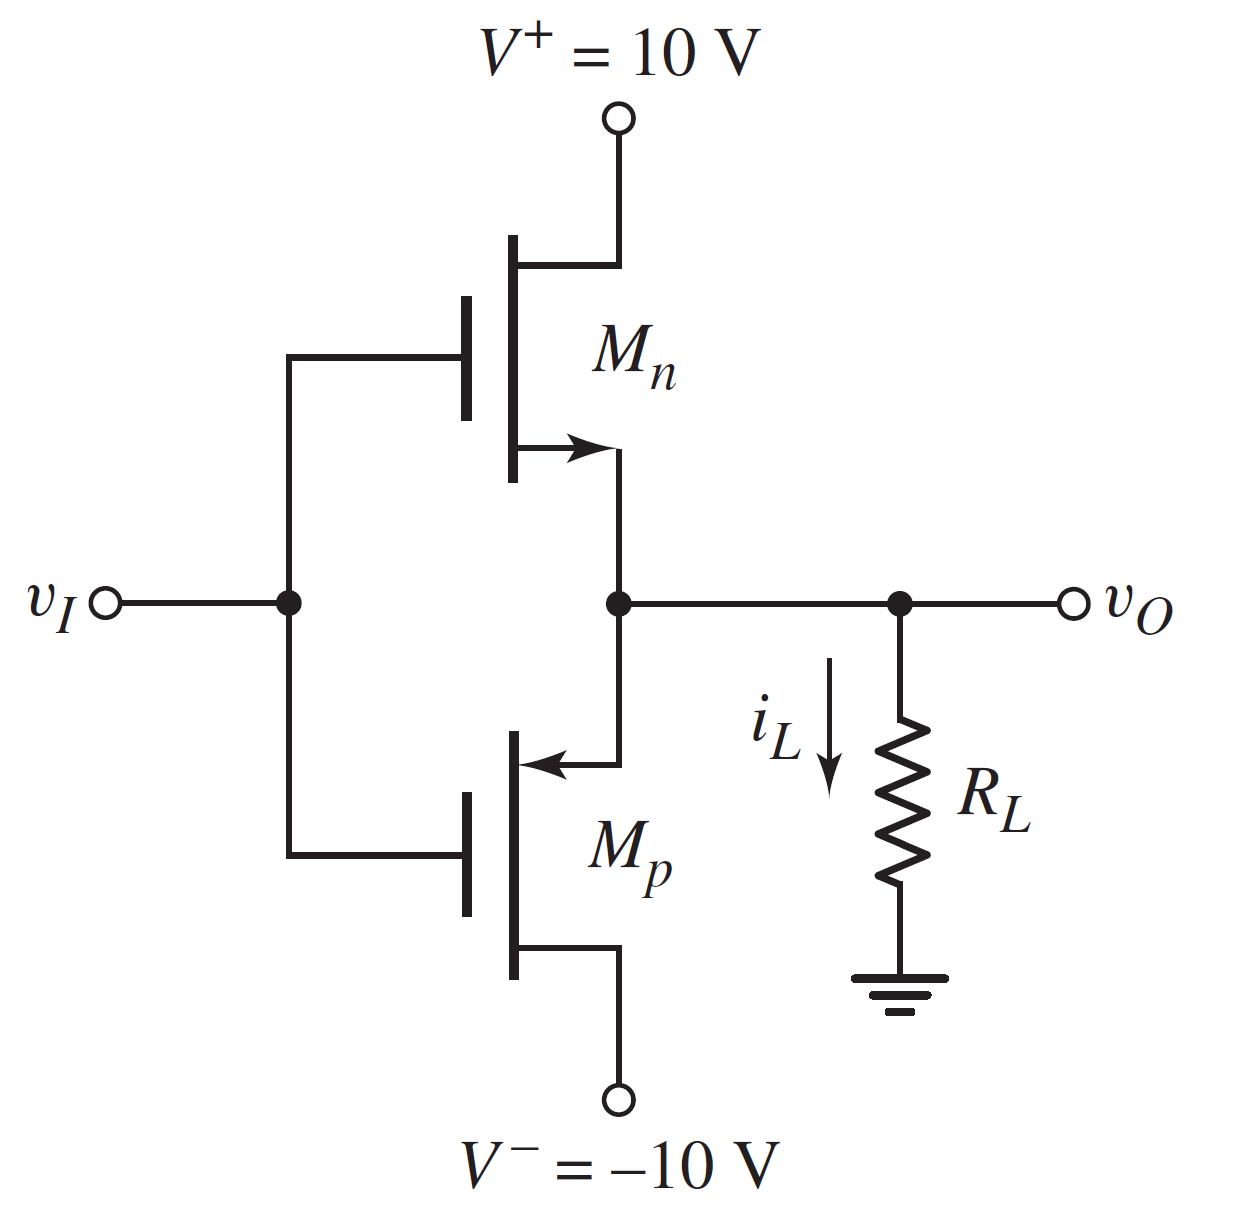
\includegraphics[width=0.5\textwidth]{8.24}
	\caption{Problem 8.24}
\end{figure}
\noindent Solution:

(a)If we want get the maximum output voltage, The $V_{DS}$ must be equal to the minimum. In fact, the minimum we can easily solve:
$$
	V_{DS{\min}}=V_{DS(sat)}=V_{GS}-V_T=V_{GS}
$$

Just consider the positive half a cycle, we have equations as follow:
$$\left\{
\begin{aligned}
	&I_D=K_nV_{GS}^2\\
	&I_D=I_L\\
	&10-V_{GS}=V_O=I_LR_L\\
\end{aligned}
\right.\Rightarrow V_O=8V
$$

So we can solve out $V_I, I_L$: 
$$
	V_I=V_O+V_{GS}=10\mathrm{V},I_L=\frac{V_O}{R_L}=1.6\mathrm{mA}
$$

(b)Average Power is follow:
$$
	\overline{P}_L=\frac{V_{o(\max)}^2}{2R_L}=6.4\mathrm{mW},\overline{P}_S=\frac{2V_SI_D}{\pi}=10.2\mathrm{mW},\eta=\frac{\overline{P}_L}{\overline{P}_S}=62.7\%
$$

8.29 An enhancement-mode MOSFET class-AB output stage is shown in Figure P8.29. The threshold voltage of each transistor is $V_{TN}=-V_{TP}=1$V and the conduction parameters of the output transistors are $K_{n1}=K_{p2}=$
5 mA/V$^{2}$. Let $I_{\text{Bias}}=200$ $\mu$ A. (a) Determine $K_{n3}=K_{p4}$ such that the quiescent drain currents in $M_1$ and $M_2$ are 5 mA. (b) Using the results of part (a), find the small-signal voltage gain $A_v=dv_O/dv_I$ evaluated at: (i) $v_O=0$, and (ii) $v_O=5$V.
\begin{figure}[H]
	\centering
	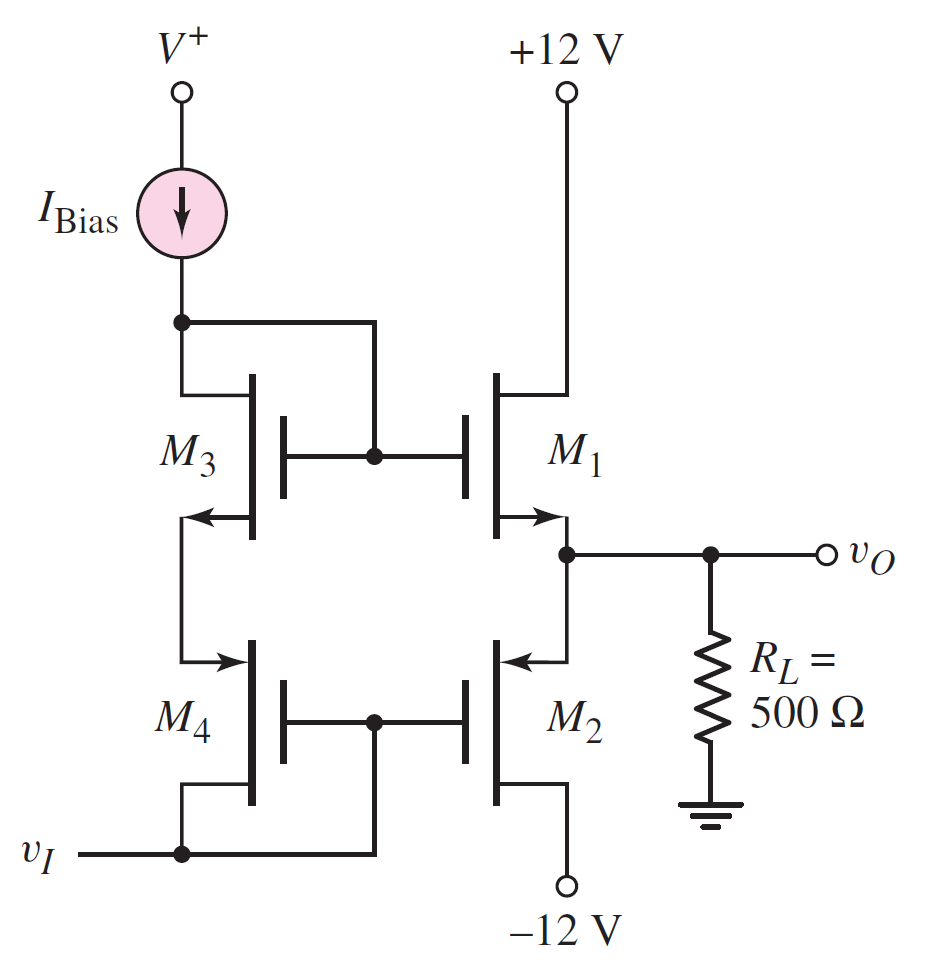
\includegraphics[width=0.5\textwidth]{8.29}
	\caption{Problem 8.29}
\end{figure}
(a)First, solve out $V_{GS1}$:
$$
	I_D=K_{n1}(V_{GS1}-1)^2\Rightarrow V_{GS1}=2\mathrm{V}
$$

Then, solve out $K_{n3}$:
$$
	I_{Bias}=K_{n3}(V_{GS1}-V_{TN})^2\Rightarrow K_{n3}=200\mu\mathrm{A/v^2}=K_{p4}
$$

(b)Because of KVL, the equation is as follow:
$$
	v_I+V_{GS3}+V_{SG4}=V_{GS1}+v_O\Rightarrow v_I+2+2=2+\sqrt{\frac{v_{o}}{R_{L}K_{n1}}}+V_{TN}
$$

Then Differentiating both sides of the equation:
$$
	1=\frac{dv_0}{dv_I}+\displaystyle\frac{1}{2\sqrt{2.5v_0}}\cdot\frac{dv_0}{dv_I}\Rightarrow \frac{dv_0}{dv_I}=\frac{2\sqrt{2.5v_0}}{2\sqrt{2.5v_0}+1}
$$

Answer is as follow:
$$v_o=0,\frac{dv_0}{dv_I}=0;v_o=5\mathrm{V},\frac{dv_0}{dv_I}=0.88$$
\end{document}